% \documentclass[12pt, twoside]{article}
\usepackage[letterpaper, margin=1in, headsep=0.2in]{geometry}
\setlength{\headheight}{0.6in}
%\usepackage[english]{babel}
\usepackage[utf8]{inputenc}
\usepackage{microtype}
\usepackage{amsmath}
\usepackage{amssymb}
%\usepackage{amsfonts}
\usepackage[nomessages]{fp} %\FPeval{\var-name}{2*sin(pi/6)}
\usepackage{siunitx} %units in math. eg 20\milli\meter
\usepackage{yhmath} % for arcs, overparenth command
\usepackage{tikz} %graphics
\usetikzlibrary{quotes, angles, arrows, arrows.meta}
\usepackage{graphicx} %consider setting \graphicspath{{images/}}
\usepackage{parskip} %no paragraph indent
\usepackage{enumitem}
\usepackage{multicol}
\usepackage{venndiagram}

\usepackage{fancyhdr}
\pagestyle{fancy}
\fancyhf{}
\renewcommand{\headrulewidth}{0pt} % disable the underline of the header
\raggedbottom
\hfuzz=2mm %suppresses overfull box warnings

\usepackage{hyperref}

\fancyhead[LE]{\thepage}
\fancyhead[RO]{\thepage \\ Name: \hspace{4cm} \,\\}
\fancyhead[LO]{BECA / Dr. Huson / Geometry\\*  Unit 8: Congruence transformations\\* 6 February 2023}

\begin{document}

\subsubsection*{7.7 Classwork: ``Onto'' mappings, symmetry}
\begin{enumerate}
\item What is the smallest non-zero angle of rotation about its center that would map the pentagon onto itself? %$ABCDE$
\begin{center}
    \begin{tikzpicture}[rotate=18, scale=1]
      \draw [thick]
      (0:2)--% node[right] {$A$}--
      (72:2)--% node[above right] {$B$}--
      (144:2)--% node[above left] {$C$} --
      (216:2)--% node[left] {$D$}--
      (288:2)--cycle;% node[right] {$E$}--cycle;
    \end{tikzpicture}
  \end{center}

\item Circle YES or NO to indicate whether the given transformation maps the hexagon onto itself.
\vspace{0.5cm}
\begin{multicols}{2}
 \begin{enumerate}
  \item Yes \quad No \quad A reflection over $\overleftrightarrow{AD}$
  \item Yes \quad No \quad A rotation of $60^\circ$ clockwise around the hexagon's center.
  \item Yes \quad No \quad A reflection over a line through the midpoints of  $\overline{BC}$, $\overline{EF}$.
  \item Yes \quad No \quad A rotation of $120^\circ$ counterclockwise around point $D$.
  \end{enumerate}
\begin{center}
    \begin{tikzpicture}%[scale=.48]
      \draw [thick]
      (0:2)node[right] {$A$}--
      (60:2)node[above right] {$B$}--
      (120:2)node[above left] {$C$} --
      (180:2)node[left] {$D$}--
      (240:2)node[left] {$E$}--
      (300:2)node[right] {$F$}--cycle;
    \end{tikzpicture}
  \end{center}
\end{multicols} \vspace{0.5cm}

\item The figure shows a rectangle (not a square).
\begin{center}
  \begin{tikzpicture}[scale=0.7]
    \coordinate (A) at (0, 0); %[label=above left:$P$]
    \coordinate (B) at (4, 0);
    \coordinate (C) at (4, 3);
    \coordinate (D) at (0, 3);
    \draw [thick] (A)--(B)--(C)--(D)--cycle;
    \draw [thick, dashed] (A)--(C);
    \draw [thick] (B)--(D);
    %\draw [thick, xshift=2cm, yshift=2.5cm] (85:3);
  \end{tikzpicture}
\end{center}
Which transformations carries the rectangle onto itself? Mark each True or False.
  \begin{enumerate}
    \item A reflection over the solid diagonal \hfill True \quad False
    \item A reflection over the dashed diagonal \hfill True \quad False
    \item A clockwise rotation of $90^\circ$ about the intersection of the diagonals \hfill True \quad False
    \item A clockwise rotation of $180^\circ$ about the intersection of the diagonals \hfill True \quad False
  \end{enumerate}

\newpage
\item A transformation maps $\triangle ABC \rightarrow \triangle DEC$, shown below. 
\begin{enumerate}
  \item Fully specify the transformation. \vspace{1cm}
\begin{multicols}{2}
  \item Identify each corresponding object. 
  \begin{enumerate}
    \item $A \rightarrow$ \rule{2cm}{0.15mm}
    \item $B \rightarrow$ \rule{2cm}{0.15mm}
    \item $C \rightarrow$ \rule{2cm}{0.15mm}
    \item $\angle ACB \cong$ \rule{2cm}{0.15mm}
    \item \rule{2cm}{0.15mm} $\cong \overline {DE}$
  \end{enumerate}
  \begin{tikzpicture}[scale=.48]
    \draw [help lines] (-2,-3) grid (9,8);
    \draw [thick, <->] (-2.4,0) -- (9.4,0) node [right] {$x$};
    \draw [thick, <->] (0,-3.4)--(0,8.4) node [above] {$y$};  
    \draw [thick]
    (4,-2) node[below left] {$A$}--
    (7,1) node[right] {$B$}--
    (1,1) node[below left] {$C$}--cycle;  
    \draw [thick]
    (4,4) node[right] {$D$}--
    (1,7) node[left] {$E$}--
    (1,1) --cycle; 
  \end{tikzpicture}
\end{multicols}
\end{enumerate}

\item Check those transformations that are rigid motions.
\begin{itemize}
  \begin{multicols}{2}
  \item[$\square$] Dilation
  \item[$\square$] Translation
  \item[$\square$] Reflection
  \item[$\square$] Rotation
  \item[$\square$] An isometry
  \item[$\square$] Horizontal stretch
  \end{multicols}
\end{itemize}

\item In the diagram below, $\triangle ABC$ with sides of 13, 15, and 17, is mapped onto $\triangle DEF$ after a clockwise rotation of $90^\circ$ about point $P$. 
\begin{multicols}{2}
  \begin{enumerate}
    \item What is $A$ mapped to? $A \rightarrow$ \vspace{1.5cm}
    \item What corresponds to $F$? \vspace{1.5cm}
    \item Given $DF=2x+1$. Find $x$. \vspace{1.5cm}
  \end{enumerate}
  \begin{tikzpicture}[scale=.6, rotate=-30]
    %\draw [thick, <->] (-7.4,0) -- (10.4,0) node [right] {$x$};
    %draw [thick, <->] (0,-5.4)--(0,10.4) node [above] {$y$};
    \fill (0,0) circle[radius=0.1] node[right]{$P$};
    \draw [thick]
      (-2,1) node[below left] {$A$}--
      (-7,2) node[left] {$B$}--
      (-4,5) node[above right] {$C$}--cycle;
      \node at (-5,1.5)[below]{17};
      \node at (-6,4){13};
      \node at (-2.5,3.5){15};
      \node at (3.25,2.25){$2x+1$};
    \draw [thick]
      (1,2) node[left] {$D$}--
      (2,7) node[above] {$E$}--
      (5,4) node[right] {$F$}--cycle;
  \end{tikzpicture}
\end{multicols}
\vspace{2cm}

\newpage
\item Reflect $\triangle TRS$ across the $y$-axis, labeling the image $\triangle T'R'S'$. Check those properties that are maintained by reflection.  \vspace{0.5cm}
\begin{multicols}{2}
  \begin{itemize}
    \item[$\square$] Length
    \item[$\square$] Angle measures
    \item[$\square$] Orientation
    \item[$\square$] Parallel relationships
    \item[$\square$] Area
  \end{itemize}
  \begin{tikzpicture}[scale=.6]
    \draw [help lines] (-7,-4) grid (7,5);
    \draw [thick, <->] (-7.4,0) -- (7.4,0) node [right] {$x$};
    \draw [thick, <->] (0,-4.4)--(0,5.4) node [above] {$y$};  
    \draw [thick]
    (4,-2) node[below left] {$T$}--
    (5,1) node[right] {$R$}--
    (2,2) node[below left] {$S$}--cycle;
  \end{tikzpicture}
\end{multicols}

\item Draw the line of reflection that would map $\triangle ABC$ onto $\triangle A'B'C'$.
\begin{center}
    \begin{tikzpicture}[rotate=100]
    %\draw [help lines] (-7,-2) grid (7,6);
    %\draw [thick, <->] (-7.4,0) -- (7.4,0) node [right] {$x$};
    %\draw [thick, <->] (0,-2.4)--(0,6.4) node [above] {$y$};  
    \draw [thick]
      (0,2) node[right] {$A$}--
      (3,4) node[left] {$B$}--
      (1,4) node[left] {$C$}--cycle;
    \draw [thick]
    (2,0) node[right] {$A'$}--
    (4,3) node[above left] {$B'$}--
    (4,1) node[right] {$C'$}--cycle;
  \end{tikzpicture}
\end{center}

\item An isometry maps $\triangle JKL \rightarrow \triangle MNO$. $m\angle K = 40^\circ$ and $m\angle M = 100^\circ$.\\[0.25cm]
  Find the measure of $\angle L$. 
\begin{flushright}
    \begin{tikzpicture}[scale=0.9]
    \coordinate [label=above left:$L$](A) at (100:2);
    \coordinate [label=below:$J$](B) at (0, 0);
    \coordinate [label=right:$K$](C) at (0:3);
    \draw [thick] (A)--(B)--(C)--cycle;
    \draw [thick, xshift=3cm, yshift=1.5cm] (100:2) node[above]{$O$}--
    (0,0) node[below]{$M$}--
    (0:3) node[right]{$N$}--cycle;
  \end{tikzpicture}
\end{flushright}

\newpage
\item Translate $\triangle DEF$ by $(x,y) \rightarrow (x+3, y-5)$. Label the image $\triangle D'E'F'$.
\begin{center}
    \begin{tikzpicture}[scale=.48]
    \draw [help lines] (-7,-5) grid (10,6);
    \draw [thick, <->] (-7.4,0) -- (10.4,0) node [right] {$x$};
    \draw [thick, <->] (0,-5.4)--(0,6.4) node [above] {$y$};  
    \draw [thick]
      (-4,4) node[below left] {$D$}--
      (3,4) node[above] {$E$}--
      (1,1) node[below] {$F$}--cycle;  
  \end{tikzpicture}
\end{center}

\item A translation maps triangle $PQR$ onto triangle $STU$. %\vspace{0.5cm}
  \begin{multicols}{2}
    \begin{tikzpicture}[scale=0.9]
      \coordinate [label=above left:$P$](A) at (95:2);
      \coordinate [label=below:$Q$](B) at (0, 0);
      \coordinate [label=right:$R$](C) at (-10:3.5);
      \draw [thick] (A)--(B)--(C)--cycle;
      \draw [thick, xshift=3cm, yshift=1.5cm] (95:2) node[above]{$S$}--
      (0,0) node[below]{$T$}--
      (-10:3.5) node[right]{$U$}--cycle;
    \end{tikzpicture}\\
    Write each corresponding object.
    \begin{enumerate}
      \item $Q \rightarrow$ \rule{2cm}{0.15mm}
      \item $\angle QRP \cong$ \rule{2cm}{0.15mm}
      \item \rule{2cm}{0.15mm} $\cong \overline {ST}$
      \item Justify $\triangle PQR \cong \triangle STU$. Use the words ``rigid motion".
    \end{enumerate}
  \end{multicols}  \vspace{1.5cm}

\item Translate $\triangle XYZ$ with $X(-1,2)$, $Y(3,4)$, $Z(1,-3)$ by $(x,y) \rightarrow (x-6, y-1)$, labeling the image $\triangle X'Y'Z'$.
\begin{center}
    \begin{tikzpicture}[scale=.48]
    \draw [help lines] (-10,-5) grid (6,6);
    \draw [thick, <->] (-10.4,0) -- (6.4,0) node [right] {$x$};
    \draw [thick, <->] (0,-5.4)--(0,6.4) node [above] {$y$};  
    \draw [thick]
      (-1,2) node[below left] {$X$}--
      (3,4) node[above] {$Y$}--
      (1,-3) node[below] {$Z$}--cycle;  
  \end{tikzpicture}
\end{center}


\end{enumerate}
\end{document}